\documentclass{scrartcl}

\usepackage[utf8]{inputenc}
\usepackage[T1]{fontenc}
\usepackage[ngerman, english]{babel}
\selectlanguage{english}
\usepackage{listings}
\usepackage{hyperref}
\usepackage{upquote}
\usepackage{graphicx}

\lstset{ %
	frame=single,
	numbers=left,
	breaklines=true,
	breakautoindent=false,
	breakatwhitespace=true,
	% keepspaces=true,
	basicstyle=\ttfamily,
	upquote=true,
}

\newcommand\solution[2]{{\paragraph{#1}#2}}
\newcommand\todo[1]{TODO: #1}


\title{Assignment 4 - Breaking WPA/Protocol implementation}
\author{$<$Simon$>$ $<$Rommer$>$, $<$1225253$>$}
\date\today{}

\begin{document}

\maketitle

\begin{abstract}
	
The year is 2020, and the entire world is using secure Wifi everywhere and
services used on the internet employ only the best protocols provided by
libraries used by millions of people. And, speaking of people, every person
uses only the most secure passwords which are impossible for machines to
crack. Well, not entirely...

The following assignment is split into two parts and it is your job to crack
the password of a WPA network and obtain privileged information you should not
have access to.

Please document your findings and your solution by filling out this template
and upload the resulting PDF to TUWEL.
\end{abstract}



\section{Breaking WPA}

\section*{Assignment}
Somewhere out there a little wifi still exists using WPA to secure connections.
As a skilled hacker you read on StackOverflow that this makes it vulnerable to
dictionary attacks. Somehow you manage to get hold of a handshake (since you of
course are also gifted in the art of social engineering). The source can't
recall the exact passphrase, but it's SSID was "wpa2own" and she remembered
that the password ended with a number (coincidentally your student ID
[Matrikelnummer]) prefixed with a password out of a famous, real-world password
list from the Internet (hint: research some famous recent hacks): [password][studentID]). You grab a coffee, warm up your
GPUs, and get ready to work ... 

\section*{Dictionary attacks}
A dictionary attack happens when an attacker tries passwords according to a given list of words (Dictionary). This doesn't even have to be a real dictionary like "Oxford Dictionary" or the "Duden". Most of the times attacker use a list of previously gained passwords from hacks. \\
Dictionary attacks can also be when you obtained a database with stored passwords as hashes and you cross reference the hashes from the passwords to the hashes you obtained.\\
The hashes from the passwordlist can be precalculated and stored in a list (a so called Rainbowtable) so that the comparison goes much faster. Also you could use graphics cards to calculate hashes since the way graphics card work make them more fitting than cpu's. (GPU achieve great performance by using heavy parallelism, possible because of pipelining and sharing instruction decoding (since many cores will run the same instructions at the same time).)\\
Countermeasures to dictionary attacks on the admin side are limiting the numbers of tries that a user has to login and set requirements for passwords. Setting requirements for passwords is not usefull if the user doesn't remember the password and chooses to use something really easy like "1234abcd".\\
Countermeasures to dictionary attacks on the user side choosing passwords that are not single words or easy numbers like "password" or "123456". Also phrases like "passw0rd" are really common. A good approach here would be to use a passwordmanager that stores all your difficult passwords. In this case you only have to remember one master-key and can have different passwords on every account. Also please don't recycle passwords.\\

If the SSID of the network is known, then the hash can be bruteforced or compared to a table. This is because of the fact that the SSID is used as the salt for the calculated hashes and the hashing function is known this makes the computational effort very low.

\section*{Approach}
The biggest challenge was to find the right password list. I used a visualization of the worlds biggest data breaches\footnote{\url{http://www.informationisbeautiful.net/visualizations/worlds-biggest-data-breaches-hacks/}}as starting point and filtered for "web" and "hacked". I checked the results for media attention and remembered that the Ashley Maddison hack had a huge media outcry becaus of the nature of the website. Even the popular TV-show "Mr.Robot" had to delay airing of an episode because of similarities to the real life event. So I googled for the Ashley Maddison-password list and found it as the second link\footnote{\url{https://github.com/danielmiessler/SecLists/blob/master/Passwords/Ashley_Madison.txt}}. \\

It was stated in the assignment that the password consists of a password of some list plus our studentID, so I wrote following short python script to add my studentID to every line in the list:

\begin{lstlisting}

with open("./pw-list/am-pass-full.txt","r") as list:

table = list.read().strip().split()
for i in range(len(table)):
table[i] = table[i] + "1225253"

with open('./pw-list/MatNr-pass.txt', mode='wt', encoding='utf-8') as myfile:
myfile.write('\n'.join(table))
\end{lstlisting}

When searching the Internet for methods of breaking a WPA-handshake you find explanations on how it works and hot to capture the handshake\footnote{\url{http://www.kalitutorials.net/2014/06/hack-wpa-2-psk-capturing-handshake.html}} and how to crack the captured handshake(which was the actual task)\footnote{\url{http://www.kalitutorials.net/2015/10/wpawpa-2-cracking-using-dictionary.html}}. \\
With a little help of a Kali-Linux VM and my friend the man-pages and some tinkering, I used following command in the KALI-bash while in the folder where I saved the data.cap and the password list:  

\begin{lstlisting}
sudo aircrack-ng -w MatNr-pass.txt -e "wpa2own" 1225253.cap
\end{lstlisting}

With the following result: \\
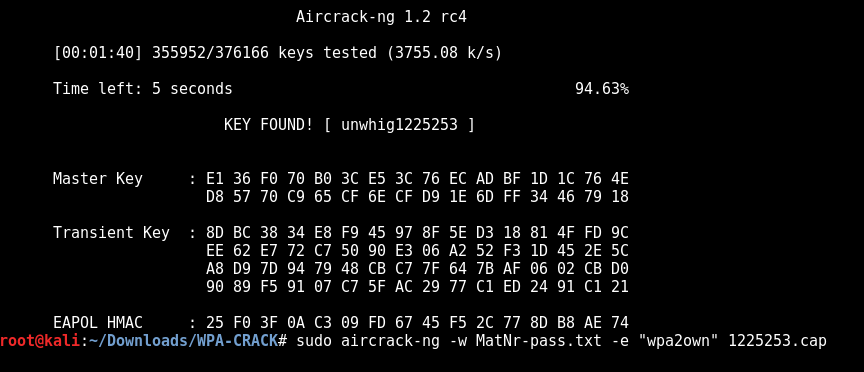
\includegraphics[scale=0.8]{passwordFound.PNG}	

And as always: \\
All the files,lists,scripts,etc. I have used can be found on my github\footnote{\url{https://github.com/Acrasy/IntroSec-WPA}}

\section*{Solutions}
\solution{WPA key}{unwhig1225253}
\solution{Password list}{modified Ashley Maddison password list\footnote{\url{https://github.com/Acrasy/IntroSec-WPA/blob/master/pw-list/MatNr-pass.txt}}}


\newpage

\section{Breaking a broken protocol}

\section*{Assignment}
After you successfully broke into the WPA network, you decide to sniff the some traffic.
As it turns out, some unknown spy agency is communicating over the same network and you find a 
reference to a secret mission request portal. You have always wanted to become a secret
agent, so you decide to participate in their next mission. Maybe they will be impressed and offer you a position.
But you do not know where the mission will be. You stare at the mission request portal and decide to hack it.

Note: You do not need to complete the first part of the assignment to solve this one.

\section*{Approach}
I remembered from a little while ago about Heartbleed and the "length" in the URL on the secret message page reminded me about this so I read up on Heartbleed and changed the value in the URL 
from 7 to a higher number. After a few random tries I came to the conclusion that length=3000 is more than enough (also I successfully tried values up until 5000 but that was really cumbersome to get valid outputs and not a segmentation-fault). \\


\section*{Exploiting the Service}
The vulnerability is that the encryption method is known and the key can be obtained because of a flaw in the database. As described a few times in this document one can read the data by changing the length of the message that is shown to a greater value. The value is not checked so the system will show as many characters as you like. Even from a certain value on the database will give back a segmentation fault, through constantly refreshing the page can the data still be obtained.\\


"Recently" in 2012 there was a bug introduced in OpenSSL that made it possible to read more data than you should allow. The bug was called "Heartbleed" because it was a faulty implementation of the TLS heartbeat extension that basically keeps two parties synchronized. The problem with the implementation is that the user input validation was faulty so you could read data by telling the database to reply with more than it should be as visualized at the xkcd comic\footnote{\url{http://xkcd.com/1354/}} that was found in the secret message page.  \\
Not validating userdata in general opens the system to all kinds of security risks like SQLi, buffer overflows and a wide range of unauthorized possibilities to tamper with the system.

\section*{Decrypting the Mission}
\solution{Mission code}{d058744a}

From the exploited mission request service it was as easy to get the encryption key as a quick site wide search for "passphrase" through the displayed text. Having the information about the encryption that was provided in the message and the passphrase, I was just a simple command away from being able to read the briefing in clear-text.
The values shown were from the memory of the database with a section that showed the passphrase for the gpg-encrypted text.   After that I opened the bash on my Windows10 box and started decrypting with following command:

\begin{lstlisting}
gpg --passphrase (passphrasehere)  --decrypt msg.txt > decoded.txt
\end{lstlisting}

This saved the decrypted message into a text-file ready for later use if needed. The message read:

\begin{quotation}
	Agent 1225253,
	
	your mission starts tomorrow. Meet us at the Cafe around the corner at 0800. Do not tell anybody. Details to follow once you arrive.
	Bring your tactical turtleneck.
\end{quotation}


\end{document}
